\chapter{Figures and Tables}
\section{Figures}
Figures are included using the code below. Remember there are environments for sideways figures and subfigures. 

\begin{figure}[tbp]
	\centering
		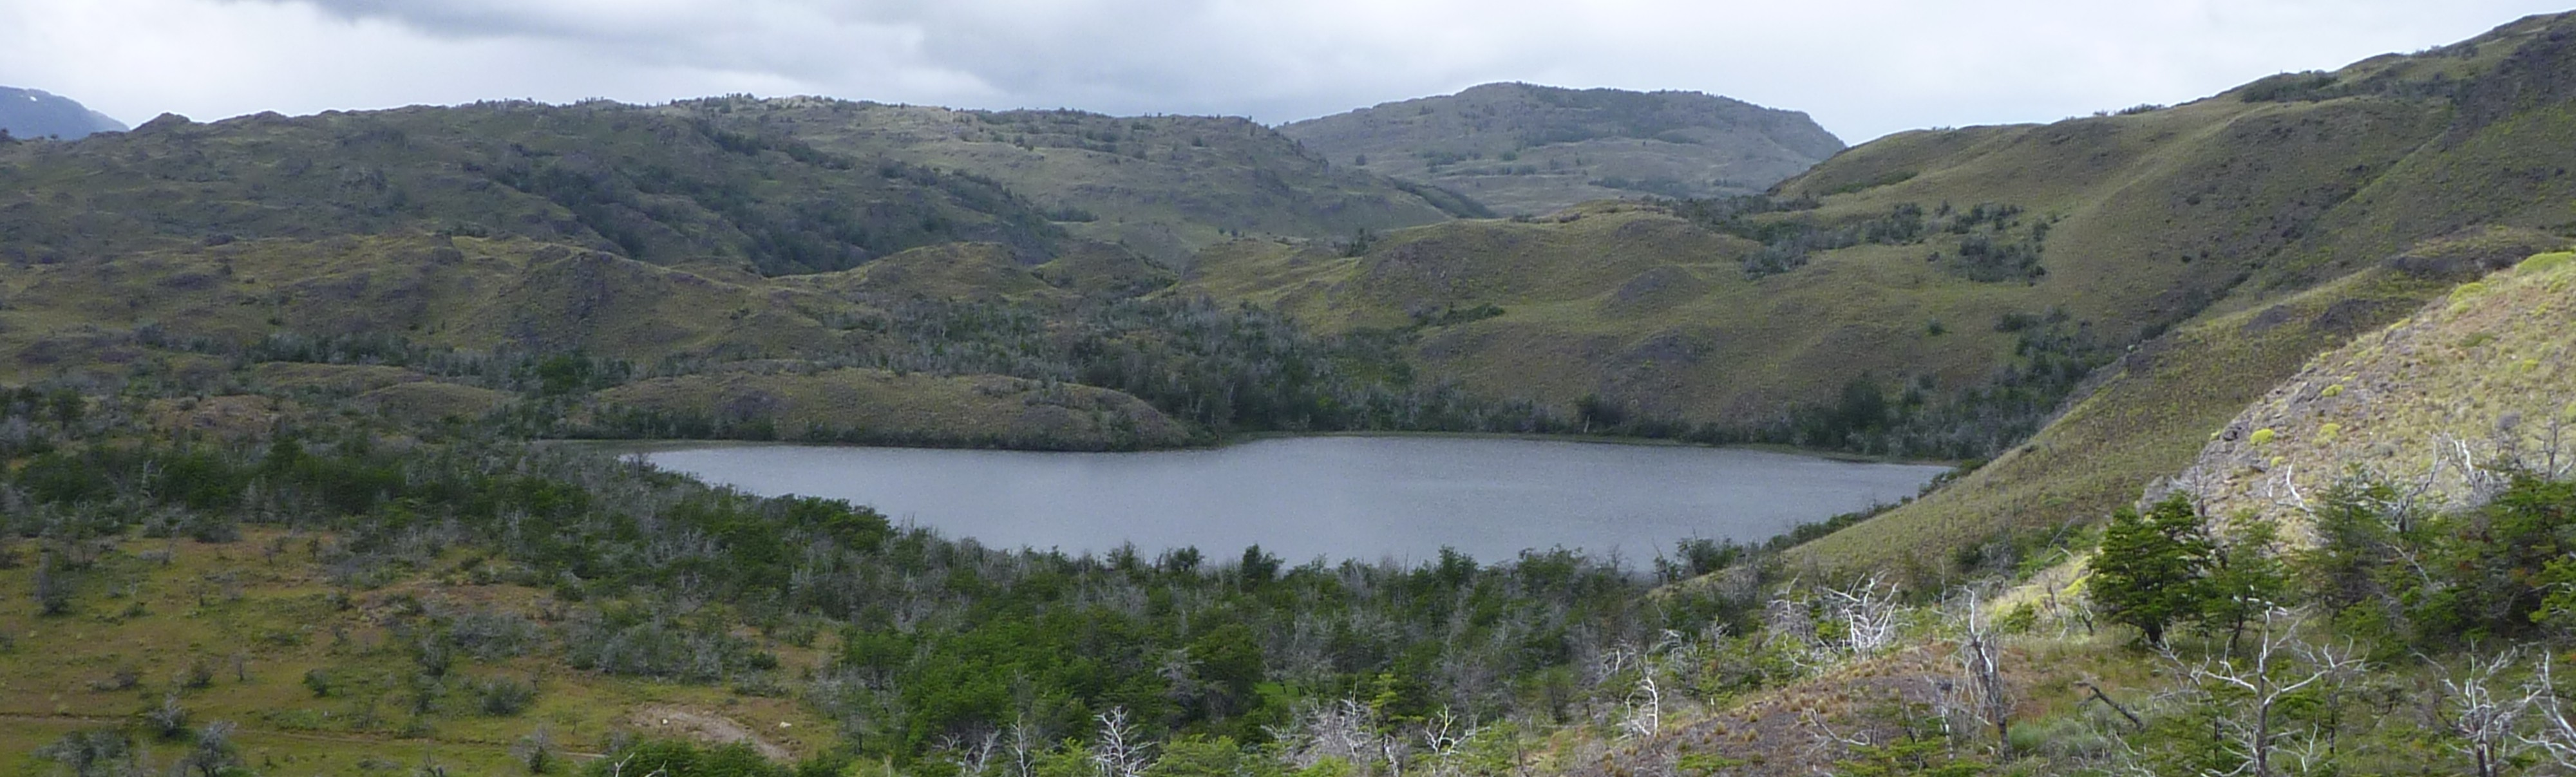
\includegraphics[width=1.00\textwidth]{edita.jpg}
	\caption[Photograph of Laguna Edita.]{Photograph of Laguna Edita, taken facing south-east.}
	\label{fig:editapic}
\end{figure}

\section{Tables}
Tables are complicated in \LaTeX. Table \ref{tab:itraxsetupsummary} is a simple example.

\begin{table}[tbp]
	\centering
		\begin{tabular}{lr}
		 \hline
		 Parameter     & Setting       \\ \hline
		 Tube          & Mo            \\
		 Voltage       & 30kV          \\
		 Current       & 30mA          \\
	   Exposure time & 30s           \\
		 Step size     & 400$\mu$m     \\
		 \hline			
		\end{tabular}
	\caption[Summary of parameters used in Itrax XRF data aquisition.]{Summary of parameters used in Itrax XRF data aquisition.}
	\label{tab:itraxsetupsummary}
\end{table}